\documentclass[expologarit]{subfiles}
\begin{document}

 \begin{center}
\color{violet} \kml លំហាត់ទី៨
 \end{center}
 គេអោយអនុគមន៍ $f$ មួយ កំណត់លើ $\mathbb{R}-\{1,3\}$ ដោយ $f(x)=\frac{x^2+4x+3}{x^2-4x+3}$។ \\
 តាង$(C)$ ជាក្រាបតាងអនុគមន៍ $f$ ក្នុងតម្រុយ$\left(O,\overrightarrow{i},\overrightarrow{j}\right)$។
 \begin{enumerate}[k]
 \item បង្ហាញថាបន្ទាត់ $y=1$ ជាសមីការអាស៊ីមតូតដេកនៃក្រាប$(C)$ ត្រង់ $\pm\infty$។\\ រួចរកសមីការអាស៊ីមតូតឈរទាំងពីរ។
 \item ចូរបង្ហាញថា $f'(x)=-\frac{8\left(x^2-3\right)}{\left(x^2-4x+3\right)^2}$ ចំពោះគ្រប់$\mathbb{R}-\{1,3\}$ ។
 \item សិក្សាអថិរភាព និងសង់តារាងអថេរភាពនៃអនុគមន៍ $f$ រួចសង់ក្រាប$(C)$។
 \item ដោយប្រើក្រាប$(C)$ ពិភាក្សាតាមតម្លៃ$k$ នូវចំនួនឫសរបស់សមីការ \\
 $(k-1)x^2-4(k+1)x+3(k-1)=0\quad (1)$\\
 រួចប្រៀបធៀបឫសរបស់ $(1)$ ទៅនឹងចំនួន $-3,\ -\sqrt{3},\ -1,\ 0,\ 1,\ \sqrt{3}$ និង $3$។
 \end{enumerate}
 \begin{center}
\color{violet} \kml ដំណោះស្រាយ
 \end{center}
  \begin{enumerate}[k]
 \item បង្ហាញថាបន្ទាត់ $y=1$ ជាសមីការអាស៊ីមតូតដេកនៃក្រាប$(C)$ ត្រង់ $\pm\infty$
\\[0.25cm]
ដោយ $\lim_{x\to \pm\infty}f(x)=\lim_{x\to \pm\infty}\frac{x^2+4x+3}{x^2-4x+3}=\lim_{x\to \pm\infty}\frac{x^2\left(1+\frac{4}{x}+\frac{3}{x^2}\right)}{x^2\left(1-\frac{4}{x}+\frac{3}{x^2}\right)}=1$ \\[0.25cm]
ដូចនេះ \fbox{បន្ទាត់ $y=1$ ជាសមីការអាស៊ីមតូតដេកនៃក្រាប$(C)$ ត្រង់ $\pm\infty$}
 \\[0.25cm] រកសមីការអាស៊ីមតូតឈរទាំងពីរ\\[0.25cm]
 ដោយ $\lim_{x\to 1}f(x)=\lim_{x\to 1}\frac{x^2+4x+3}{x^2-4x+3}=\pm\infty$\\[0.25cm]
 ហើយ
 $\lim_{x\to 3}f(x)=\lim_{x\to 3}\frac{x^2+4x+3}{x^2-4x+3}=\pm\infty$\\[0.25cm]
 ដូចនេះ \fbox{បន្ទាត់ $x=1$ និង $x=3$ ជាអាស៊ីមតូតឈរនៃក្រាប$(C)$}
 \newpage 
 \item បង្ហាញថា $f'(x)=-\frac{8\left(x^2-3\right)}{\left(x^2-4x+3\right)^2}$ ចំពោះគ្រប់$\mathbb{R}-\{1,3\}$ 
 \begin{flalign*}
 f'(x)=\left(\frac{x^2+4x+3}{x^2-4x+3}\right)'&=\frac{(2x+4)\left(x^2-4x+3\right)-\left(2x-4\right)\left(x^2+4x+3\right)}{\left(x^2-4x+3\right)^2}&\\
 &=\frac{-8x^2+24}{\left(x^2-4x+3\right)^2}=-\frac{8\left(x^2-3\right)}{\left(x^2-4x+3\right)^2}
 \end{flalign*}
 ដូចនេះ \fbox{$f'(x)=-\frac{8\left(x^2-3\right)}{\left(x^2-4x+3\right)^2}$ ចំពោះគ្រប់$\mathbb{R}-\{1,3\}$ }
 \item សិក្សាអថិរភាព 
\\ ដោយ  $f'(x)=-\frac{8\left(x^2-3\right)}{\left(x^2-4x+3\right)^2}$ \\
យើងបាន $f'(x)=0\Leftrightarrow\quad -8\left(x^2-3\right)=0 \quad\Leftrightarrow\quad -8x^2+24=0\quad \Rightarrow x=\pm\sqrt{3}$\\
 តារាសញ្ញាដេរីវេ $f'(x)$
\\[0.2cm]
\begin{tikzpicture}
   \tkzTabInit[lw=1,lgt=1.5,espcl=2]{$x$ / 0.75 , $f'(x)$ / 1}{$ -\infty$ , $-\sqrt{3}$,$1$,$\sqrt{3}$,$3$, $+\infty $}
   \tkzTabLine{, -, z,+,d, + , z, -, d ,- }
\end{tikzpicture}
\begin{itemize}
\item $f'(x)>0$ ឬ អនុគមន៍ $f$ កើន ពេល $x\in\left(-\sqrt{3},1\right)\cup\left(1,\sqrt{3}\right)$
\item $f'(x)<0$ ឬ អនុគមន៍ $f$ ចុះ ពេល $x\in\left(-\infty ,-\sqrt{3}\right)\cup\left(\sqrt{3},3\right)\cup\left(3,+\infty\right)$
\end{itemize}
បរមាធៀប
\begin{itemize}
\item ត្រង់ $x=-\sqrt{3};\ f'(x)=0$ ហើយប្តូរសញ្ញាពី$-$ទៅ$+$ នោះ $f$ មានអប្បបរមាធៀបមួយគឺ 
\begin{flalign*}
f(-\sqrt{3})&=\frac{\left(-\sqrt{3}\right)^2+4\left(-\sqrt{3}\right)+3}{\left(-\sqrt{3}\right)^2-4\left(-\sqrt{3}\right)+3}=4\sqrt{3}-7 &
\end{flalign*}
\item ត្រង់ $x=\sqrt{3};\ f'(x)=0$ ហើយប្តូរសញ្ញាពី$+$ទៅ$-$ នោះ $f$ មានអតិបរមាធៀបមួយគឺ 
\begin{flalign*}
f(\sqrt{3})&=\frac{\left(\sqrt{3}\right)^2+4\left(\sqrt{3}\right)+3}{\left(\sqrt{3}\right)^2-4\left(\sqrt{3}\right)+3}=-4\sqrt{3}-7 &
\end{flalign*}
\end{itemize}
សង់តារាងអថិរភាពនៃអនុគមន៍ $f$ 
\\[0.2cm]
\begin{tikzpicture}
   \tkzTabInit[lw=1,lgt=1.5,espcl=2]{$x$ / 0.75 , $f'(x)$ / 1,$f(x)$/2}{$ -\infty$ , $-\sqrt{3}$,$1$,$\sqrt{3}$,$3$, $+\infty $}
   \tkzTabLine{, -, z,+,d, + , z, -, d ,- }
       \tkzTabVar{+/ $1$,-/$4\sqrt{3}-7$ ,+D-/ $+\infty$/ \ $-\infty$ ,+/$-4\sqrt{3}-7$, -D+/ $-\infty$ / \ $+\infty$, -/ $1$}
\end{tikzpicture}
\\
សង់ក្រាប$(C)$
\begin{flalign*}
(C)\cap (x'ox)\Leftrightarrow\quad y=0\quad &\Leftrightarrow\quad  x^2+4x+3=0\Rightarrow x_1=-1,\ x_2=-3 &\\
 (C)\cap (y'oy)\Leftrightarrow\quad x=0\quad & \Rightarrow\quad  y=\frac{0^2+4(0)+3}{0^2-4(0)+3}=1\\
 (C)\cap (d):y=1\quad\Leftrightarrow\quad\quad   & 1 =\frac{x^2+4x+3}{x^2-4x+3}\\
 \quad\Leftrightarrow\quad \quad  & x^2-4x+3 =x^2+4x+3\quad \Rightarrow x=0
\end{flalign*}

 \begin{center}
\begin{tikzpicture}[x=1cm,y=1cm]
\begin{axis}[scale=1,
          xmax=15.5,ymax=8.5,
          axis lines=middle,
          xmin=-8.5,ymin=-16.5,          
          xtick={-13,-11,...,15},
          ytick={-15,-10,...,10}  ,
          xlabel=$x$   ,
          ylabel=$y$   ,x=0.5cm, y=0.25cm
          ] 
\addplot[domain=-13:15.5 ,restrict y to domain=-19:14,line width=1pt,samples=1000,smooth,name path=A,color=red] {(x^2+4*x+3)/(x^2-4*x+3)};
\addplot[domain=-14.5:15.5,line width=1.5pt,samples=100,smooth] {1}node[sloped, near end,above]{$y=1\qquad\qquad$};

%\addplot [color=black]coordinates {(-2.5,0)} node[below ]{$x'$};

%\node at(0,-1){$\bullet$};

%\draw[dashed](1,0)--(1,1)--(0,1);

             %\addplot[gray, pattern=north west lines] fill between[of=A and B, soft clip={domain=1:2}];
            

       
        
  
              \draw (0,0)rectangle (0.2,0.2);
           
             \draw[line width=1.5pt] (1,-19)--(1,14)node[sloped, near end,below]{$x=3$};
                          \draw[line width=1.5pt] (3,-19)--(3,14)node[sloped, near end,below]{$x=-4$};
            \draw (5,8) node {$(C)$};
             \draw (1,0) node {$\bullet$};
              \draw (-1,0) node {$\bullet$};
               \draw (-3,0) node {$\bullet$};
              \draw (0,1) node {$\bullet$};
              \draw[dashed] (1.73,0)--(1.73,-13.93)node{$\bullet$}--(0,-13.93);
                \draw[dashed] (-1.73,0)--(-1.73,-0.07)node{$\bullet$}--(0,-0.07);
              
\end{axis}
\end{tikzpicture}
 \end{center}
 \item  ពិភាក្សាតាមតម្លៃ$k$ នូវចំនួនឫសរបស់សមីការ 
 $(k-1)x^2-4(k+1)x+3(k-1)=0\quad (1)$
 \begin{flalign*}
 (1)\Leftrightarrow\quad & kx^2-x^2-4kx-4x+3k-3=0 & \\
  \Leftrightarrow\quad   &  k\left(x^2-4x+3\right)-\left(x^2+4x+3\right)=0\\
  \Leftrightarrow\quad & k=\frac{x^2+4x+3}{x^2-4x+3} \\
  \Leftrightarrow\quad & k=f(x) \quad \text{ជាសមីការអាប់ស៊ីសរវាងក្រាប$(C)$និងបន្ទាត់ $y=k$}
 \end{flalign*}
  តាមក្រាប$(C)$ 
  \begin{itemize}
  \item បើ $k\in\left(-\infty ,-4\sqrt{3}-7\right)\qquad\qquad\Rightarrow (1)$ មានឫសពីរផ្សេងគ្នាដែល $1<x_1<x_2<3$
  \item បើ $k=-4\sqrt{3}-7\qquad\qquad\qquad \ \ \Rightarrow (1)$ មានឫសតែមួយគត់ $x=\sqrt{3}$
  \item បើ $k\in\left(-4\sqrt{3}-7,4\sqrt{3}-7\right)\quad\ \  \Rightarrow (1)$ គ្មានឫស
  \item បើ $k=4\sqrt{3}-7 \qquad\qquad\qquad\ \ \ \ \Rightarrow (1)$ មានឫសតែមួយគត់គឺ $x=-\sqrt{3}$
  \item បើ $k\in\left(4\sqrt{3}-7,1\right)\qquad\qquad\quad\ \ \Rightarrow (1)$ មានឫសពីរផ្សេងគ្នា ដែល  $x_1<x_2<0$
  \item បើ $k=1 \qquad\qquad\qquad\qquad \ \ \ \ \ \ \ \ \Rightarrow (1)$ មានឫសតែមួយគត់ គឺ $x=0$
  \item បើ $k\in\left(1,+\infty\right)\qquad\qquad\qquad \ \ \ \ \Rightarrow (1)$ មានឫសពីរផ្សេងគ្នាដែល $0<x_1<1\ ;\quad 3<x_2$ 
  \end{itemize}

 \end{enumerate}
\end{document}